

\section{Forelesning 15: (Mandag \date{24. februar 2025})}
\subsection{Poissons equation at the unit square on a regular grid}

Let \(\Omega = [0,1]\times[0,1]\) and \(\mathcal{L}u = \Delta u = u_{xx} + u_{yy} = f\).
\begin{align*}
  \mathcal{L}u & = f \quad \text{on} \quad \Omega = (0,1) \times (0,1) \\
  u            & = g \quad \text{on} \quad \partial\Omega_D
\end{align*}

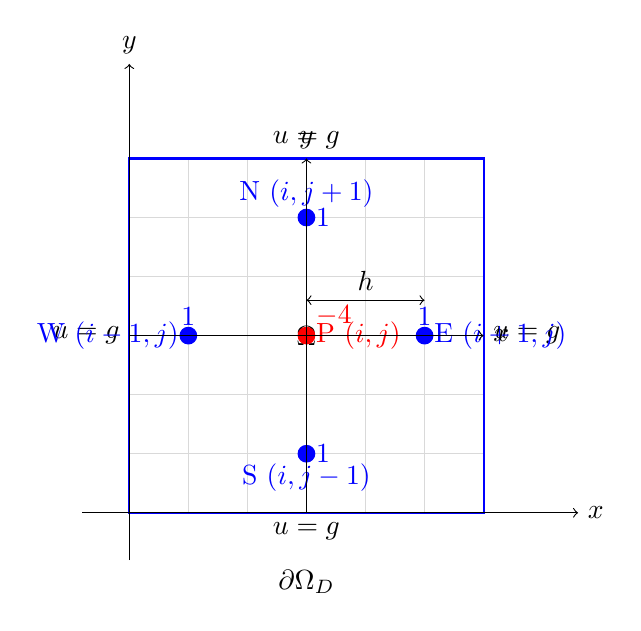
\begin{tikzpicture}[scale=1.5]
  % Grid 
  \draw[step=0.5cm,gray!30] (0,0) grid (3,3);
  % Domain blue boundary at the unit square
  \draw[thick,blue] (0,0) rectangle (3,3);
  % Axes
  \draw[->] (-0.4,0) -- (3.8,0) node[right] {$x$};
  \draw[->] (0,-0.4) -- (0,3.8) node[above] {$y$};
  % Label domain
  \node at (1.5,1.5) {$\Omega$};
  \node[below] at (1.5,-0.4) {$\partial\Omega_D$};
  % Label boundary conditions
  \node[left] at (0,1.5) {$u=g$};
  \node[right] at (3,1.5) {$u=g$};
  \node[below] at (1.5,0) {$u=g$};
  \node[above] at (1.5,3) {$u=g$};

  % Center point and neighbors (P = point, N = north, S = south, E = east, W = west)
  \filldraw[red] (1.5,1.5) circle (2pt) node[right] {P $(i,j)$};
  \filldraw[blue] (2.5,1.5) circle (2pt) node[right] {E $(i+1,j)$};
  \filldraw[blue] (1.5,2.5) circle (2pt) node[above] {N $(i,j+1)$};
  \filldraw[blue] (0.5,1.5) circle (2pt) node[left] {W $(i-1,j)$};
  \filldraw[blue] (1.5,0.5) circle (2pt) node[below] {S $(i,j-1)$};

  % Connect points with lines
  \draw[gray,dashed] (0.5,1.5) -- (2.5,1.5);
  \draw[gray,dashed] (1.5,0.5) -- (1.5,2.5);

  % Coefficient labels
  \node[red] at (1.5,1.5) [above right] {$-4$};
  \node[blue] at (2.5,1.5) [above] {$1$};
  \node[blue] at (1.5,2.5) [right] {$1$};
  \node[blue] at (0.5,1.5) [above] {$1$};
  \node[blue] at (1.5,0.5) [right] {$1$};

  % Mesh size label
  \draw[<->] (1.5,1.8) -- (2.5,1.8) node[midway,above] {$h$};

  % Coordinate axes
  \draw[->] (0,1.5) -- (3,1.5) node[right] {$x$};
  \draw[->] (1.5,0) -- (1.5,3) node[above] {$y$};

\end{tikzpicture}
\paragraph{5 point formula}
Central Difference Operator for \(u_{xx} + u_{yy}\):
\[
  \Delta u = = \frac{1}{h^2}\left(u_{i+1,j} + u_{i,j+1} + u_{i-1,j} + u_{i,j-1} - 4u_{i,j}\right)
\]

\paragraph{Error Analysis}
Want to find an upper bound for the error.

\[
  \abs{e_{i,j}} = \abs{u_{i,j} - U_{i,j}} \leq C_1h^2 + C_2h^4 \quad p\in \mathring{\Omega}_h
\]

\subparagraph{Local Truncation Error}
\begin{align*}
  \tau_p = \mathcal{L}_h u_p - f_p                                \\
  \mathcal{L}_h u_p = f_p \quad \forall p \in \mathring{\Omega}_h \\
  \mathcal{L}_h u_p = \tau_p \quad \forall p \in \partial\Omega_h
\end{align*}

Use the \emph{Max Discrete Principle} to show that the error is bounded by the local truncation error.

\subparagraph{Max Discrete Principle}
Let \(\mathcal{L}u = u_{xx} + u_{yy}\) on \(\Omega \in \R^2\), where \(\Omega\) is open and connected. And let \(v\) be a sufficiently smooth function on \(\overline{\Omega} = \Omega \cup \partial\Omega\).

if \(\mathcal{L}u \geq 0\) on \(\Omega\) and \(u = v\) on \(\partial\Omega\), then
\[
  v \leq \max_{\partial\Omega} v
\]

if \(\mathcal{L}u \leq 0\) on \(\Omega\) and \(u = v\) on \(\partial\Omega\), then
\[
  v \geq \min_{\partial\Omega} v
\]

if \(\mathcal{L}u = 0\) on \(\Omega\) and \(u = v\) on \(\partial\Omega\), then both minimum and maximum are attained on the boundary.
\[
  \mathcal{L}u = 0 \quad \forall p \in \mathring{\Omega}_h
\]

\paragraph{The discrete maximum principle (5-point formula)}

Given \(\{v_p\}_{p \in \Omega_h}\) and let
\[
  \mathcal{L}_h v_p = \frac{1}{h^2}\left(v_E + v_N + v_W + v_S - 4v_P\right) \quad p \in \overline{\Omega}_h
\]
\begin{itemize}
  \item If \(\mathcal{L}_h v_p \geq 0\) for all \(p \in \Omega_h\) for all \(p \in \overline{\Omega}_h\), then
        \[
          v_P \leq \max_{R \in \partial\Omega_h} v_R
        \]
  \item If \(\mathcal{L}_h v_p \leq 0\) for all \(p \in \Omega_h\) for all \(p \in \overline{\Omega}_h\), then
        \[
          v_P \geq \min_{R \in \partial\Omega_h} v_R
        \]
\end{itemize}

\begin{proof}{By contradiction}{}
  Assume that there is one point \(p^\star\) s.t. \(v_{p^\star} \geq V_p \forall p \in \overline{\Omega}_h\),
  but then
  \[
    v_p^\star \geq v_{E^\star}, v_{N^\star}, v_{W^\star}, v_{S^\star}
  \]
  from
  \[
    \delta_h v_{p^\star} \geq 0 \implies 4v_{p^\star} \leq v_{E^\star} + v_{N^\star} + v_{W^\star} + v_{S^\star} \leq 4v_{p^\star}
  \]
  This can only be true if \(v_{p^\star} = v_{E^\star} = v_{N^\star} = v_{W^\star} = v_{S^\star}\),
  Continue this argument for one neighbor point and continue until a boundary point is reached.

  \textbf{Two cases:}
  \begin{itemize}
    \item[a)] \(v_p\) is constant for all \(p \in \overline{\Omega}_h\) and then \(\mathcal{L}_h v_p = 0\).
    \item[b)] or \(\max_{p \in \overline{\Omega}_h} v_p = \max_{R \in \partial\Omega_h} v_R\).
  \end{itemize}
\end{proof}

\paragraph{Local Truncation Error}

\begin{align*}
  \tau_p = \mathcal{L}_h u_p - f_p = \mathcal{L}_h u_p - \mathcal{L}u_p                                                                                 \\
  \mathcal{L}_h U_p = \frac{1}{h^2}\left(\delta_x^2 U_p + \delta_y^2 U_p\right), \quad p = (x_i, y_j) \in \mathring{\Omega}_h                           \\
  \tau_p = \frac{1}{h^2}\left(\delta_x^2 u_p + \delta_y^2 u_p\right)                                                                                    \\
  \tau_p = \delta_x^2 u_p - \frac{h^2}{12}\partial_x^4 u(x_i + \xi_i h, y_j) + \delta_y^2 u_p - \frac{h^2}{12}\partial_y^4 u(x_i, y_j + \eta_j h) - f_p \\
  \tau_p = - \frac{h^2}{12}\left(\partial_x^4 u(x_i + \xi_i h, y_j) + \partial_y^4 u(x_i, y_j + \eta_j h)\right), \quad \xi_i, \eta_j \in (-1, 1)       \\
  K = \max\{ \max_{\Omega} \abs{\partial_x^4 u}, \max_{\Omega} \abs{\partial_y^4 u}\}                                                                   \\
  \abs*{\tau_p} \leq \frac{h^2}{12} K = \overline{\tau}                                                                                                 \\
  e_p = u_p - U_p                                                                                                                                       \\
  \boxed{\mathcal{L}_h e_p = \tau_p, \quad p \in \mathring{\Omega}_h \text{ and } e_R = 0, \quad R \in \partial\Omega_h}
\end{align*}

Search for a \(\phi\) to lift the error \(e_p\) s.t. the maximum principle holds.

Properties of \(\phi\):

\begin{align*}
  \mathcal{L}_h \phi_p = \mathcal{L} \phi_p = 0 \quad (\phi \in \mathbb{P}_3)                                                                                                                                     \\
  \mathcal{L} \phi = 1 \text{ or some other constant, e.g. } \phi \in \mathbb{P}_2                                                                                                                                \\
  \mathcal{L}_h(e_p + \overline{\tau}\phi) = \tau_p + \overline{\tau} \geq 0                                                                                                                                      \\
  e_p + \tau \phi_p \overset{\text{apply 1st DMP}}{\leq} \max_{R \in \partial\Omega_h}\{e_R + \tau \phi_R\} = \overline{\tau}\max_{R \in \partial\Omega_h}\phi_R \leq \overline{\tau} \max_{\partial\Omega_h}\phi \\
  e_p \leq \overline{\tau}\left(\max_{R \in \partial\Omega_h}\phi_R - \phi_p\right) \leq \overline{\tau}\left(\max_{\partial\Omega_h}\phi - \min_{\partial\Omega_h}\phi\right)                                    \\
\end{align*}

\subparagraph{Better error estimate}
\begin{align*}
  \phi = \frac{1}{4}\left[(x - \tfrac{1}{2})^2 + (y - \frac{1}{2})^2\right] \implies \abs*{e_p} \leq \frac{h^2}{48}K \\
  \mathcal{L}_h \left(e_p - \overline{\tau}\phi_p\right)\leq 0                                                       \\
  \boxed{\abs*{e_p} \leq \overline{\tau}\left(\max_{\partial\Omega_h}\phi - \min_{\overline{\Omega}_h}\phi\right)}   \\
  \text{BO: } \phi = \frac{1}{2}x^2 \implies \mathcal{L}_h \phi = 1, \; \mathcal{L}_h \phi = \mathcal{L} \phi = 0    \\
  \max_{\partial\Omega_h}\phi = \frac{1}{2} \quad \min_{\overline{\Omega}_h}\phi = 0                                 \\
  \boxed{\abs*{e_p} \leq \frac{h^2}{12}K} \quad \text{where} K = \max_{\Omega} \{\abs{\partial_x^4 u}, \abs{\partial_y^4 u}\}
\end{align*}


